\documentclass[11pt, a4paper]{article}
\usepackage[utf8]{inputenc}
\usepackage{bookmark}
\usepackage[margin=1in]{geometry} 
\usepackage{amsmath,amsthm,amssymb}
\usepackage[margin=1in]{geometry} 
\usepackage{amsmath,amsthm,amssymb}
\usepackage{multicol}
\usepackage[slovene]{babel}
\usepackage{color}
\usepackage{graphicx}
\usepackage{amssymb}
\usepackage{amsmath}
\usepackage{mathtools}
\usepackage{commath}
\usepackage{ragged2e}
\usepackage[T1]{fontenc}
\usepackage[normalem]{ulem}
\usepackage{amsthm}
\usepackage{esvect}
\usepackage{float}
\usepackage{calrsfs}
\usepackage{tocloft}
\DeclareMathAlphabet{\pazocal}{OMS}{zplm}{m}{n}
\newcommand{\Ga}{\mathcal{G}}


\newcommand\setItemnumber[1]{\setcounter{enumi}{\numexpr#1-1\relax}}


\newtheorem{theorem}{Trditev}[section]
\newtheorem{corollary}{Posledica}[section]
\newtheorem{lemma}[section]{Lema}
\theoremstyle{definition}
\newtheorem{definition}{Definicija}[section]
\theoremstyle{example}
\newtheorem{example}[section]{Primer}
\theoremstyle{izrek}
\newtheorem{izrek}[section]{Izrek}
\begin{document}
\begin{figure}[H]
    \centering
    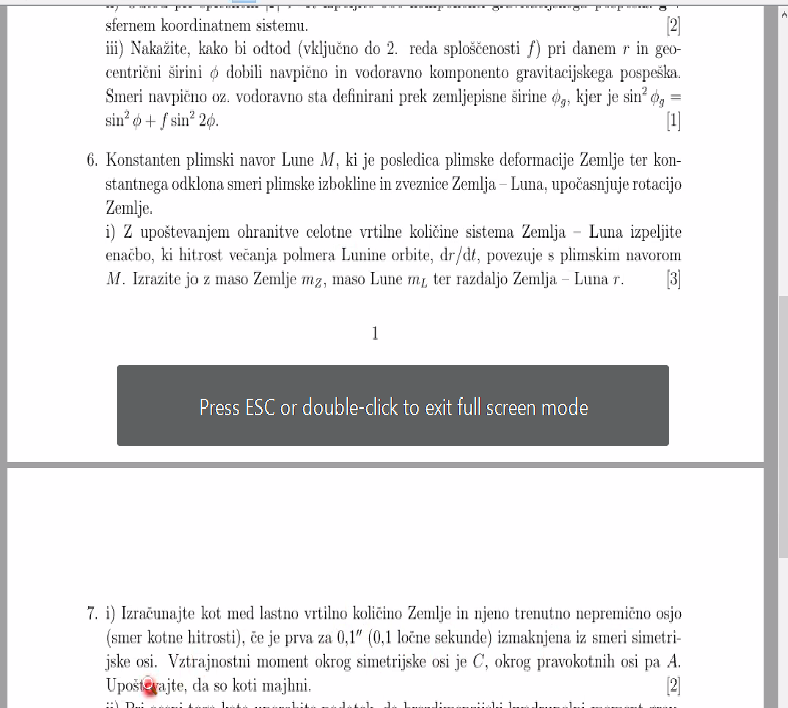
\includegraphics[width=17cm, height=20cm]{Screenshot 1.png}
    \caption{Prikaz postavitve meritve}
\end{figure}
\pagebreak
\begin{figure}[H]
    \centering
    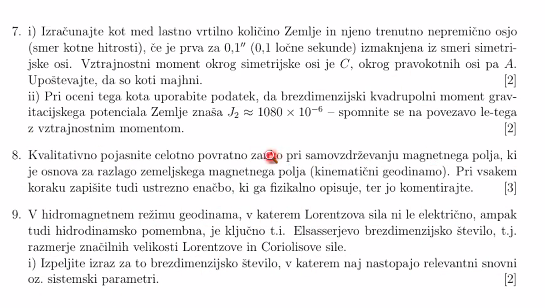
\includegraphics[width=17cm, height=20cm]{Screenshot 2.png}
    \caption{Prikaz postavitve meritve}
\end{figure}

\pagebreak


$$U_1=\pi \nu B (r_2^2-r_1^2)=\frac{\pi}{2}V$$

$$U_i=\frac{d\Phi}{dt}=\frac{BdS}{dt}=\frac{Br^2}{2}\frac{d\phi }{dt}$$

$$U_i=\pi B \nu r^2=0.235 V$$


$$U_i=v B l \cos(\phi) \qquad \phi=\frac{2\pi}{t_0}t$$
$$U_i=\frac{2 \pi}{t_0}Blr \cos(\frac{2 \pi}{t_0}t)=1.26 V \cdot \cos(\frac{2 \pi}{t_0}t)$$


$$U_i=NBS\frac{M}{J}t \sin(\frac{M}{J}t^2) \qquad t^2=\frac{2 \pi N J}{M}$$
\begin{center}
ker je $\omega=\frac{M}{J}t$.

\end{center}


$$I(t)=\frac{B(ab+ad)S}{t \zeta l}=\frac{B(ab+ad)S}{t \zeta (3a+2b+2d)}=0.13 A$$

$$\frac{m c_v \Delta T}{t}=P=U_I I$$
$$\Delta T=t\frac{B^2\pi^2 r^4 \omega^2}{2 R m c_v}$$

\pagebreak
$$U_i=\frac{d}{dt}\frac{I(t)\mu_0 a}{2 \pi}\ln(\frac{b+a}{b-a})$$
$$I=I_0 e^{i\omega t}(1-e^{i\delta})$$

$$P=\frac{U^2}{R}=$$

$$|I|^2=I\cdot I^{*}=I_0^2 e^{i\omega t}e^{-i \omega t}(1-e^{i \delta})(1-e^{-i \delta})=I_0^2 (1-e^{i \delta}-e^{-i \delta}+1)=I_0^2 (2-e^{i \delta}-e^{-i \delta})=2I_0^2(1-\cos(\delta))$$

\pagebreak
$$P=U_0 \cos(\omega t) \frac{U_0}{|Z|}\cos(\omega t -\delta)$$

$$\cos(\omega t -\delta)=\cos(\omega t) \cos(\delta)+\sin(\omega t)\sin(\delta)$$
$$\sin(2x)=2\sin(x)\cos(x)$$
$$P=\frac{U_0^2}{|Z|}(\cos(\delta) \cos^2(\omega t)+\frac{1}{2}\sin(\delta)\sin(2\omega t))\quad \rightarrow \quad\frac{U_0^2}{2|Z|}\cos(\delta)$$

Drug način:
$$P=\frac{U_0^2}{|Z|}e^{(i\omega t-i\delta)}\cdot e^{i\omega t}$$
$$e^{(i\omega t-i\delta)}\cdot e^{i\omega t}=e^{i(2\omega t-\delta}$$

\pagebreak
$$P_{el}=P_{Q}$$
$$j_{el}S=j_Q S'$$
$$j_{el}\pi r^2 =j_Q 2\pi rl$$
$$j_{el} r =-\lambda \frac{dT}{dr} 2 l$$

$$j_{el}=\frac{P_{el}}{S_0}=\frac{UI}{S_0}=\frac{I^2R}{S_0}=\frac{I^2 \zeta l}{ S_0^2 }$$

$$\frac{I^2 \zeta l}{ S_0^2 } r =-\lambda \frac{dT}{dr} 2 l$$
\begin{center}
FUCKING KOŠNIK:

\end{center}
$$P_{el}=P_Q$$
$$\frac{P_{el}}{V}=q_{el}=\frac{UI}{V}=\frac{I^2R}{V}=\frac{I^2\zeta}{S^2}=j^2 \zeta$$
$$q_{el} V=j_Q S$$

$$q_{el} \pi r^2 l=j_Q 2\pi rl $$
$$q_{el} r=-2\lambda \frac{dT}{dr}$$

$$\int_{0}^{r_1} q_{el} r dr=-2\lambda \int_{T_1}^{T_2} dT$$
$$\frac{q_{el}r_1^2}{2}=-2\lambda (T_2-T_1)$$
\begin{center}
Sedaj vstavimo, da je $q_{el}=\frac{I^2\zeta}{S^2}$

\end{center}
$$\frac{I^2\zeta r_1^2}{2S^2}=-2\lambda (T_2-T_1)$$
$$I=\sqrt{\frac{4\lambda(T_1-T_2)S^2}{\zeta r_1^2}}$$
\end{document}

